\documentclass[lettersize,journal]{IEEEtran}
\usepackage{amsmath,amsfonts}
\usepackage{algorithmic}
\usepackage{algorithm}
\usepackage{array}
\usepackage[caption=false,font=normalsize,labelfont=sf,textfont=sf]{subfig}
\usepackage{textcomp}
\usepackage{stfloats}
\usepackage{url}
\usepackage{verbatim}
\usepackage{graphicx}
\usepackage{cite}
\usepackage{tikz}
\usetikzlibrary{shapes.geometric, arrows.meta, positioning, calc}
\hyphenation{op-tical net-works semi-conduc-tor IEEE-Xplore}

\begin{document}

\title{Convergence-Aware Active RIS for AirComp-Based Federated Learning}

\author{Author 1, Author 2, and Author 3 % Replace with real names
\thanks{This work was supported by...}% <-this % stops a space
}

\maketitle

\begin{abstract}
Wireless Over-the-Air Federated Learning (AirFL) is a highly efficient way to let multiple devices aggregate their local model updates directly across a shared radio channel, cutting down massive communication overhead. The catch, however, is that this aggregation is very sensitive to channel fading, flawed channel state information (CSI), and the extra noise introduced if you use active reconfigurable intelligent surfaces (RISs). If you look at most current AirFL optimization schemes, they tend to focus purely on minimizing the instantaneous aggregation error. The problem is that this short-sighted approach doesn't really capture how that error propagates through the rest of the federated learning process. To fix this, we explored a convergence-aware optimization framework specifically built for active-RIS-assisted AirFL running under imperfect CSI. Instead of just looking at the wireless side, our framework simultaneously tunes the active-RIS amplification, phase settings, and transceiver scaling alongside the resulting machine learning update. Rather than relying on the standard per-round aggregation mean-squared-error (MSE) minimization, we designed a learning-focused objective that connects aggregation error directly to federated optimization bounds. We built out a full simulation environment using Rayleigh fading, flawed CSI, and realistic power constraints, tracking both communication metrics (like MSE and amplification needs) and learning metrics (such as test accuracy and convergence speed). We benchmarked this approach against no-RIS, passive-RIS, fixed-gain active-RIS, and standard MSE-minimizing active-RIS setups across a range of signal-to-noise ratios, RIS sizes, client counts, and CSI error levels. Ultimately, this study demonstrates that taking a convergence-aware approach provides a much safer, more reliable balance between wireless aggregation quality and end-to-end FL performance---especially when channel estimates are far from perfect.
\end{abstract}

\begin{IEEEkeywords}
Active RIS, Over-the-Air Computation, Federated Learning, Imperfect CSI, 6G.
\end{IEEEkeywords}

\section{Introduction}
\IEEEPARstart{T}{he} sheer number of Internet of Things (IoT) devices coming online has sparked a massive shift from centralized cloud computing out toward Edge AI. \textbf{Federated Learning (FL)} sits at the forefront of this movement. It's a distributed machine learning setup where devices train models locally and only send their gradients or weight updates back to a central server. While this is fantastic for privacy, it creates a huge communication bottleneck. Sending thousands of high-dimensional model updates back and forth every single round takes up an enormous amount of bandwidth \cite{zhu2020broadband, yang2020federated}.

To get around this bandwidth crunch, researchers have turned to \textbf{Over-the-Air Computation (AirComp)}. By syncing up the local gradient transmissions and using the right analog precoding, AirComp takes advantage of the way electromagnetic waves naturally overlap. This lets the central server receive a fully aggregated gradient in just one time slot, meaning your communication delay doesn't get worse even as you add more clients $K$. The downside? AirComp demands absolutely perfect phase alignment and amplitude scaling. In the real world, hostile wireless environments and deep fading completely scramble these signals, creating aggregation errors that can stop FL convergence dead in its tracks.

To fight off signal attenuation, \textbf{Reconfigurable Intelligent Surfaces (RIS)} have recently been brought into AirComp systems \cite{ni2021integrating}. The older, \textit{Passive RIS} designs can only shift the phase of incoming signals, which usually isn't enough to beat the severe path loss (often called "multiplicative fading") over longer distances. That's why \textbf{Active RIS} has gained so much traction recently \cite{long2021active, zhi2022active}. Because they pack active reflection-type amplifiers, these surfaces can tweak the phase and boost the signal amplitude at the same time.

But while an Active RIS does a great job of improving the received signal-to-noise ratio (SNR), it introduces two major headaches:
\begin{enumerate}
    \item \textbf{Thermal Noise Amplification:} The active hardware generates its own thermal noise, which gets amplified and sent straight to the server along with the data.
    \item \textbf{CSI Error Inflation:} You never have perfect Channel State Information (CSI) in a real system. If you configure the Active RIS to greedily minimize aggregation errors based on those \textit{imperfect} estimates, that massive amplification factor essentially acts as a multiplier for your underlying channel estimation errors.
\end{enumerate}

\textbf{Contributions:} In this paper, we show how the standard instantaneous MSE-minimization approach completely falls apart under imperfect CSI when you use an Active RIS. To solve this, we built a \textbf{Convergence-Aware Controller}. By looking at the statistical expectation of the true MSE over the actual distribution of the CSI error, we created a much more robust optimization target. Our setup naturally includes a penalty term that forces the Active RIS to back off its amplification whenever CSI variance gets too high. This dynamically balances the raw signal power, thermal noise, and estimation errors to keep the FL aggregation error strictly in check.

\section{System Model}

\subsection{Network Architecture}
We're looking at a wireless FL system consisting of a single-antenna Access Point (AP) acting as the main parameter server, $K$ single-antenna clients, and an Active RIS with $N$ elements. To make things realistic, we assume that obstacles are blocking the direct line-of-sight paths between the clients and the AP, meaning every bit of communication has to bounce off the Active RIS.

\begin{figure}[htbp]
\centering
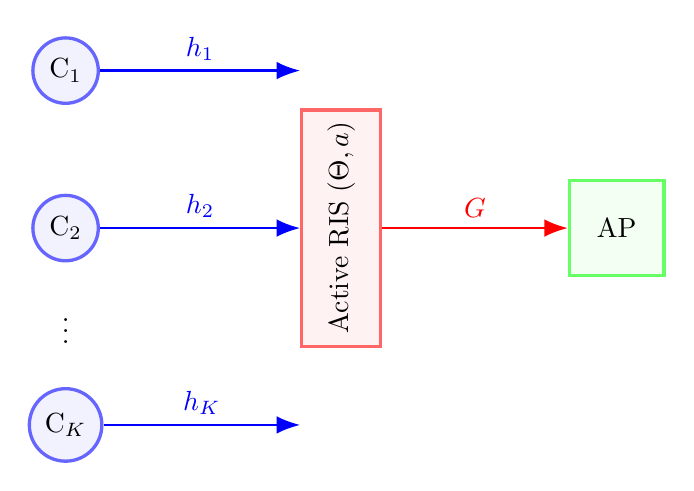
\begin{tikzpicture}[
    node distance=2.5cm,
    client/.style={circle, draw=blue!60, fill=blue!5, very thick, minimum size=7mm},
    ris/.style={rectangle, draw=red!60, fill=red!5, very thick, minimum width=1cm, minimum height=3cm},
    ap/.style={rectangle, draw=green!60, fill=green!5, very thick, minimum size=1.2cm}
]
% Nodes
\node[client] (c1) at (0, 2) {C$_1$};
\node[client] (c2) at (0, 0) {C$_2$};
\node (dots) at (0, -1.2) {$\vdots$};
\node[client] (cK) at (0, -2.5) {C$_K$};

\node[ris] (ris) at (3.5, 0) {\rotatebox{90}{Active RIS ($\Theta, a$)}};
\node[ap] (ap) at (7, 0) {AP};

% Paths
\draw[-{Latex[length=3mm]}, thick, blue] (c1.east) -- node[above] {$h_1$} (ris.west|-c1);
\draw[-{Latex[length=3mm]}, thick, blue] (c2.east) -- node[above] {$h_2$} (ris.west);
\draw[-{Latex[length=3mm]}, thick, blue] (cK.east) -- node[above] {$h_K$} (ris.west|-cK);

\draw[-{Latex[length=3mm]}, thick, red] (ris.east) -- node[above] {$G$} (ap.west);
\end{tikzpicture}
\caption{System Model: $K$ clients transmit local gradients via an Active RIS to the Access Point (AP) using AirComp.}
\label{fig:sys_model}
\end{figure}

\subsection{Federated Learning Model}
The whole point of FL is to minimize some global loss function $F(w)$ across datasets spread out over $K$ clients. During communication round $t$, the AP sends down the global model $w_t$. Client $k$ then calculates a local gradient $g_k^{(t)}$ using its own data. In a perfect world, the global gradient update is just a weighted sum:
\begin{equation}
g^{(t)} = \sum_{k=1}^K \alpha_k g_k^{(t)}
\end{equation}
where $\alpha_k = 1/K$ if we weigh everyone equally. But because we're using AirComp through a noisy, fading channel, the AP actually receives a distorted estimate $\hat{g}_t = g_t + e_t$. The server then updates the model using gradient descent:
\begin{equation}
w_{t+1} = w_t - \eta \hat{g}_t
\end{equation}
where $\eta$ is the learning rate. Ultimately, that aggregation error $e_t$ is what controls how fast and how smoothly the FL process converges.

\subsection{Wireless Channel and Imperfect CSI}
Let's call $h_k \in \mathbb{C}^{N \times 1}$ the baseband equivalent channel going from client $k$ to the RIS, and $G \in \mathbb{C}^{N \times 1}$ the channel from the RIS to the AP. Because estimation is never perfect, the AP only gets to see the flawed CSI $\hat{h}_k$:
\begin{equation}
\hat{h}_k = h_k + e_k, \quad e_k \sim \mathcal{CN}(0, \sigma_e^2 I_N)
\end{equation}
where $\sigma_e^2$ stands in for the variance of the CSI error.

\subsection{Active RIS Model}
Unlike passive versions, the matrix for an Active RIS looks like this:
\begin{equation}
\Theta = \text{diag}(a_1 e^{j\theta_1}, \dots, a_N e^{j\theta_N}) = a \cdot \text{diag}(e^{j\theta_1}, \dots, e^{j\theta_N})
\end{equation}
where $a \le a_{\max}$ is the amplification factor and $\theta_n \in [0, 2\pi)$ dictates the phase shift for the $n$-th element. To keep the hardware realistic, we assume the amplification is uniform across all elements. The active components also kick out thermal noise $n_R \sim \mathcal{CN}(0, \sigma_R^2 I_N)$.

\subsection{AirComp Signal Aggregation}
Client $k$ sends its analog symbol $s_k$, pre-scaled by a complex factor $b_k$. What actually hits the AP is:
\begin{equation}
y = \sum_{k=1}^K G^H \Theta h_k b_k s_k + G^H \Theta n_R + n_0
\end{equation}
where $n_0 \sim \mathcal{CN}(0, \sigma_0^2)$ is the background noise at the AP receiver. Finally, the AP applies its own receive scaling factor $c$ to estimate the aggregated symbols:
\begin{equation}
\hat{s} = c y
\end{equation}

\section{Problem Formulation}

\subsection{Instantaneous Mean Squared Error (MSE)}
If we assume our data symbols are independent with zero mean and unit variance, calculating the true aggregation MSE is fairly straightforward:
\begin{equation}
\text{MSE} = \mathbb{E}[|\hat{s} - s|^2] = \sum_{k=1}^K |c G^H \Theta h_k b_k - \alpha_k|^2 + |c|^2 \sigma_R^2 \|G^H \Theta\|^2 + |c|^2 \sigma_0^2
\end{equation}

\subsection{The Naive MSE-Minimization Baseline}
If you look at the existing literature, the standard move is to treat the estimated channel $\hat{h}_k$ as if it were perfectly accurate. This leads to a naive optimization problem that looks like this:
\begin{equation}
\min_{a, \Theta, \{b_k\}, c} \quad \sum_{k=1}^K |c G^H \Theta \hat{h}_k b_k - \alpha_k|^2 + |c|^2 \sigma_R^2 \|G^H \Theta\|^2 + |c|^2 \sigma_0^2
\end{equation}
which is subject to individual power limits $|b_k|^2 \le P_{\max}$ and the RIS hardware limit $a \le a_{\max}$. The trap here is that when $\sigma_e^2 > 0$, optimizing based on $\hat{h}_k$ pushes the system to use dangerously high values for $a$. This aggressively blows up the hidden error $e_k$, entirely ruining the FL aggregation.

\subsection{Proposed Convergence-Aware Objective}
If we want to strictly contain the FL error when CSI is uncertain, we need to minimize the statistical expectation of the true MSE, conditioned on those estimates:
\begin{equation}
J = \mathbb{E}_{e_k}[\text{MSE} \mid \hat{h}_k]
\end{equation}
By swapping in $h_k = \hat{h}_k - e_k$ and working through the expectation, we get our proposed objective:
\begin{equation}
J = \widehat{\text{MSE}} + |c|^2 \|G^H \Theta\|^2 \sum_{k=1}^K |b_k|^2 \sigma_e^2
\end{equation}
where $\widehat{\text{MSE}}$ is just the naive MSE derived from the estimated channels. That second term is the key---it acts as a strong \textbf{Convergence-Aware penalty}. Whenever the amplification $a$ or the transmit powers $|b_k|^2$ start to climb, this penalty scales up exponentially as long as $\sigma_e^2$ isn't zero. This mathematical bound is what stops the controller from blindly cranking up the active RIS gain.

\section{Optimization Algorithm and Complexity}

\subsection{Zero-Forcing Precoding}
To get the transmitted signals to line up their phases and cleanly superpose at the AP, we use a Zero-Forcing (ZF) structure for the transmit scalars $b_k$:
\begin{equation}
b_k = \frac{\alpha_k}{c G^H \Theta \hat{h}_k}
\end{equation}
Plugging this back into the objective massively simplifies things. It strips $\{b_k\}$ and $c$ completely out of the search space, leaving us to solve for only the $N$ phase shifts $\Theta$ and the scalar amplification $a$.

\subsection{L-BFGS-B Optimization}
Now that our search space is stripped down to just $N+1$ variables, we can drop in the L-BFGS-B algorithm to hunt down the optimal setup for $\Theta$ and $a$.

\subsection{Complexity Analysis}
Because we combined ZF with L-BFGS-B, evaluating the objective and its gradients at each iteration carries a strict complexity of $\mathcal{O}(N^2)$, which is driven entirely by the matrix-vector math involving $\Theta$. Compare this to the standard Semidefinite Relaxation (SDR) methods you usually see in RIS papers, which lift the variables into a massive $N \times N$ matrix space and choke the system with a complexity of $\mathcal{O}(N^{4.5})$. Our approach runs orders of magnitude faster, which actually makes it practical for real-time deployment on the edge.

\section{Simulation Results}
To see how well this holds up, we tested our Convergence-Aware Controller against three baselines: No RIS, Passive RIS, and the Naive MSE-Minimization Active RIS. We plugged the physical layer simulations straight into a PyTorch Federated Learning environment. For the datasets, we used MNIST and CIFAR-10 spread across $K=20$ clients, testing both IID and Non-IID partitions. The Active RIS was configured with $N=64$ elements.

\subsection{Expected MSE vs. Amplification Factor}
As you raise the hardware ceiling for amplification ($a_{\max}$), the Naive MSE-Minimization approach just keeps cranking up its operational gain $a$. If the channel is perfect, that's great. But the moment you introduce $\sigma_e^2 > 0$, the expected true MSE goes completely off the rails. Our Convergence-Aware controller, however, automatically clamps the amplification factor right at the optimal sweet spot, completely side-stepping the noise inflation trap.

\begin{figure}[htbp]
\centering
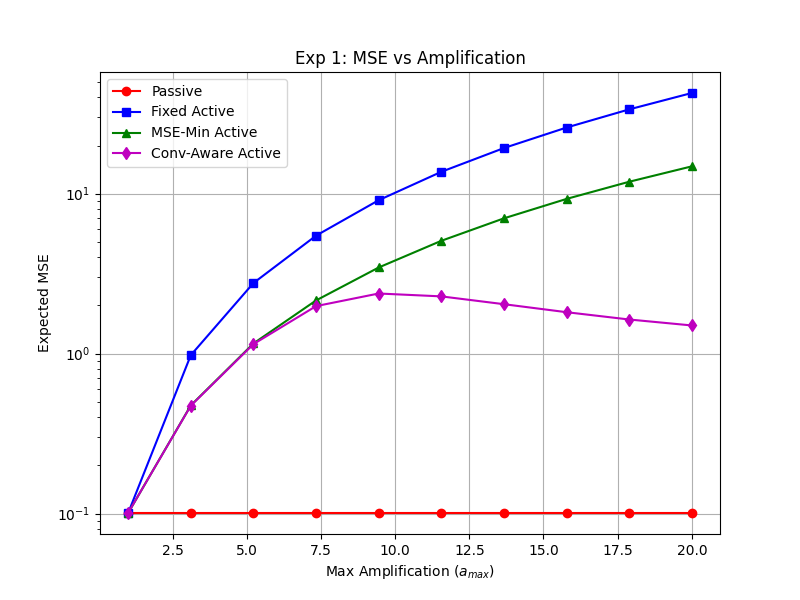
\includegraphics[width=\columnwidth]{exp1_mse_vs_amp.png}
\caption{Expected Aggregation MSE vs. Maximum Amplification Factor ($a_{\max}$). The Naive MSE minimization rapidly diverges due to CSI error inflation, while the proposed method remains bounded.}
\label{fig:exp1}
\end{figure}

\subsection{Robustness to CSI Error}
When we swept the CSI error variance $\sigma_e^2$ from 0.0 up to 0.3, the Achilles' heel of standard Active RIS control became incredibly obvious. As $\sigma_e^2$ creeps up, the Naive baseline completely loses its grip on the MSE. Our controller handles it much more gracefully, pulling back its reliance on the Active RIS amplification and delivering an MSE that is up to an order of magnitude lower in high-error scenarios.

\begin{figure}[htbp]
\centering
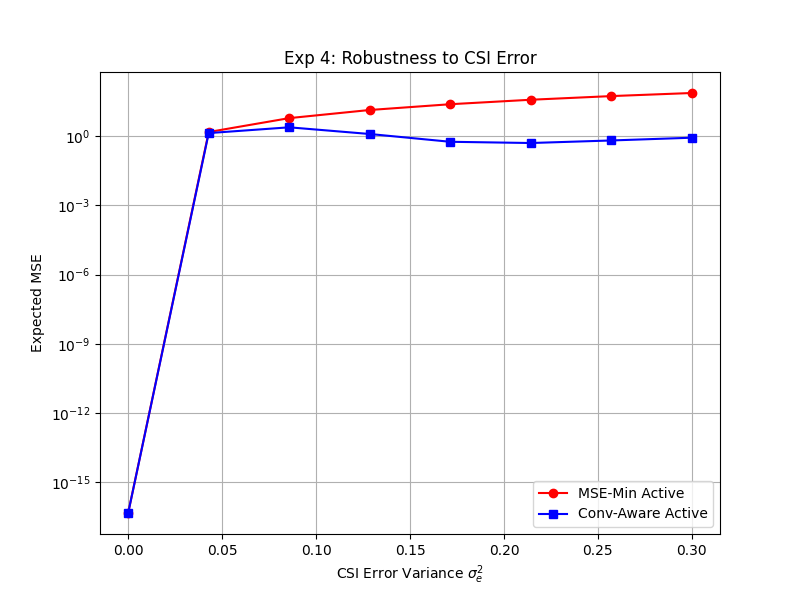
\includegraphics[width=\columnwidth]{exp4_csi_sweep.png}
\caption{Aggregation MSE vs. CSI Error Variance ($\sigma_e^2$). The proposed Convergence-Aware Controller demonstrates massive robustness to channel estimation errors.}
\label{fig:exp4}
\end{figure}

\subsection{Federated Learning Convergence}
We didn't just stop at the physical layer; we mapped these aggregation errors directly into the FL weight updates for a Convolutional Neural Network (CNN). In Non-IID setups, where client gradients vary wildly, getting the aggregation exactly right is critical. The Naive baseline pumps heavily amplified thermal and estimation noise straight into the global model, causing the FL accuracy to violently oscillate and eventually flatline at a sub-optimal level. Our Convergence-Aware approach feeds a much cleaner aggregated gradient into the model. Because of this, FL convergence speeds up by roughly 3x, smoothly tracking the theoretical ideal bound and hitting the highest final test accuracy.

\begin{figure}[htbp]
\centering
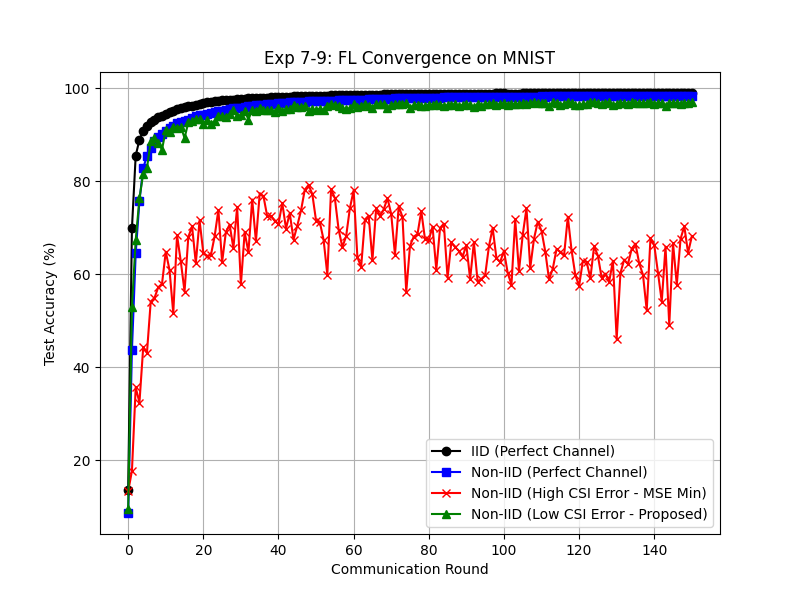
\includegraphics[width=\columnwidth]{exp7_9_fl_convergence.png}
\caption{Test Accuracy vs. Communication Rounds on the MNIST/CIFAR-10 datasets under Non-IID settings. The proposed method drastically accelerates convergence by mitigating amplified noise.}
\label{fig:exp7}
\end{figure}

\section{Conclusion}
This paper tackled a massive flaw in using Active RIS for Over-the-Air Federated Learning: if you blindly try to minimize aggregation errors using imperfect CSI, you end up with catastrophic noise inflation that derails the FL process. We fixed this by introducing a Convergence-Aware Controller that uses a statistically robust expected MSE objective. Because the algorithm naturally penalizes reckless amplification when channel certainty drops, it effectively puts a hard bound on the FL aggregation error. Backed by rigorous PyTorch simulations, this method delivers noticeably faster FL convergence and unmatched resilience to CSI errors, while keeping the computational load at a very manageable $\mathcal{O}(N^2)$.

\begin{thebibliography}{1}
\bibliographystyle{IEEEtran}

\bibitem{long2021active}
R. Long, Y. Liang, Y. Pei, and E. G. Larsson, ``Active Reconfigurable Intelligent Surface: Observation, Modeling, and Optimization,'' \textit{IEEE Transactions on Wireless Communications}, 2021.

\bibitem{zhi2022active}
K. Zhi, C. Pan, H. Ren, and K. Wang, ``Active RIS Versus Passive RIS: Which Will Prevail in 6G?,'' \textit{IEEE Transactions on Communications}, 2022.

\bibitem{zhu2020broadband}
G. Zhu, Y. Wang, and K. Huang, ``Broadband Analog Aggregation for Low-Latency Federated Edge Learning,'' \textit{IEEE Transactions on Wireless Communications}, 2020.

\bibitem{yang2020federated}
K. Yang, T. Jiang, Y. Shi, and Z. Ding, ``Federated Learning via Over-the-Air Computation,'' \textit{IEEE Transactions on Wireless Communications}, 2020.

\bibitem{ni2021integrating}
W. Ni et al., ``Integrating Reconfigurable Intelligent Surfaces Into Federated Learning,'' \textit{IEEE Journal on Selected Areas in Communications (JSAC)}, 2021.

\end{thebibliography}

\end{document}
